\documentclass[manuscript]{aastex62}
\usepackage{amsmath}
\usepackage{mathtools}
\usepackage{color}
\usepackage[normalem]{ulem}

\newcommand\latex{La\TeX}
\newcommand{\dd}{{\mathrm d}}
\newcommand{\rmsub}[1]{_\mathrm{#1}}
\newcommand{\bmu}{\boldsymbol{\mu}}
\newcommand{\beps}{\boldsymbol{\varepsilon}}
\newcommand{\blam}{\boldsymbol{\Lambda}}
\newcommand{\vx}[1]{{\bf {#1}}}
\newcommand{\vxhat}[1]{{\bf {\hat{#1}}}}

\graphicspath{{./}{figures/}}

\shorttitle{Multiplicative linear nuisance parameters}
\shortauthors{Tchernyshyov}

\begin{document}

\title{Analytic marginalization of absorption line continua and other multiplicative linear nuisance parameters}

\author[0000-0003-0789-9939]{Kirill Tchernyshyov}
\affiliation{Department of Physics and Astronomy, Johns Hopkins University, 3400 N. Charles Street, Baltimore, MD 21218, USA}
\correspondingauthor{Kirill Tchernyshyov}
\email{ktcherny@gmail.com}

%\author[0000-0003-4797-7030]{J. E. G. Peek}
%\affiliation{Department of Physics and Astronomy, Johns Hopkins University, 3400 N. Charles Street, Baltimore, MD 21218, USA}
%\affiliation{Space Telescope Science Institute, 3700 San Martin Drive, Baltimore, MD 21218, USA}

\begin{abstract}
absorption line fitting; speeding it up; well-motivated ways of selecting parameters; large spectroscopic surveys
\end{abstract}

\keywords{methods: statistical}

\section{Introduction}
\label{sec:introduction}
The formation and measurement of many astronomical observables involves processes that combine multiplicatively rather than additively.
Light from a distant source is attenuated by intervening interstellar matter (ISM) on its way to a detector; the output of the detector has to be converted to physically meaningful units by applying calibration factors.
Often, only some of the multiplicative processes represented in an observable are relevant to a study.
Attenuation by the ISM is a confounding variable for a study of a stellar populations based on a color magnitude diagram; the intrinsic spectral energy distribution of a star is a confounding variable in a study of the shape of the interstellar extinction curve.
When using Bayesian inference to learn about the relevant processes, it is necessary to marginalize over the parameters describing the confounding processes.
Because this marginalization can be time consuming if done using a numerical method such as Markov chain Monte Carlo (MCMC), it is advantageous to marginalize over nuisance parameters analyticly whenever this is possible.
We have created a package, \texttt{name}\footnote{available \emph{here}}, for analyticly marginalizing over nuisance parameters that enter an observable multiplicatively and linearly (multiplicative linear nuisance parameters or MLNPs).

The problem this package is designed for is the analysis of absorption features in spectra.
The process by which a spectrum containing absorption features is formed is the first example we gave in the paragraph above: a source emits light which is then attenuated by intervening matter.
The unattenuated light is customarily called \emph{the continuum}.
To determine parameters describing the intervening matter, it is necessary to also determine parameters describing the continuum.
While it is possible to pre-determine the continuum parameters using a portion of the spectrum that does not contain absorption features, we prefer to infer the absorption feature and continuum parameters simultaneously in order to explicitly include the uncertainty in continuum placement in estimates of the absorption feature parameters.
This is also the approach used in the recently released absorption line analysis packages \texttt{Starfish}, \texttt{sick}, and \texttt{BayesVP} \citep{2015ApJ...812..128C,2016ApJS..223....8C,Liang:2018kq}.
In these packages, absorption feature and continuum parameters are simultaneously marginalized over using MCMC.
The authors of both packages point out that marginalizing over large numbers of continuum parameters in this way can lead to long convergence and autocorrelation times.
To keep the number of continuum parameters low, the packages either do not support (\texttt{BayesVP}) or advise against (\texttt{sick}) including continuum parameters when simultaneously analyzing multiple spectral segments.

If the continuum is a linear function of the continuum parameters, the prior on the continuum parameters is (multivariate) normal or improper uniform, and the likelihood function of the observed spectrum given a model spectrum is multivariate normal, the necessary marginalization can be done analytically instead of numerically.
The key is that when the absorption feature parameters are held fixed, the continuum basis elements, the transmittance spectrum, and, if necessary, the line spread function (LSF) can be combined into a single design matrix.
The problem becomes equivalent to the simple linear nuisance parameter model discussed in an astronomical context in \citet{2017RNAAS...1a...7L}.
The likelihood marginalized over the continuum parameters is available in e.g. \citet{Rasmussen:2006vz} for both the normal prior and the improper uniform prior cases.

Analytic marginalization over multiplicative linear nuisance parameters has been used for other problems in astronomy.
In one common use case, the parameter that is marginalized over is the amplitude of a signal whose shape is a non-linear function of some parameters of interest.
One example of this use case is \citet{2017ApJ...837...20P}, where the parameters of interest are the period, eccentricity, phase, and argument of the radial velocity curve of a potential binary system and the nuisance parameters are the velocity amplitude of the curve and the barycenter velocity of the system.
Another example can be found in \citet{Leistedt:2017in}, where the parameter of interest is the redshift of a galaxy  and the nuisance parameter is the galaxy's luminosity.
This problem is not identical to the ones discussed in our paper and in \citet{2017ApJ...837...20P} because the luminosity multiplies both the data and the covariance matrix of the model residuals.
The resulting marginal likelihood can not be expressed in terms of commonly used functions.
The concept, however, is analogous and an accurate analytic approximation is available.

When developing this package, we were specifically considering properties of the absortion spectrum likelihood function and useful ways in which it can be factored.
The mathematical contribution of this work is an expression for the gradient of the logarithm of the marginal likelihood with respect to the problem's interesting non-linear parameters.
This gradient can be used for optimization or in gradient-aware sampling methods such as Hamiltonian Monte Carlo \citep{DUANE1987216}.
The other contribution is the package itself, which uses the structure of the likelihood function to efficiently calculate the marginal likelihood and gradient.
We state the problem and give expressions for the marginal likelihood and the gradient of its logarithm in Section \ref{sec:assumptions-and-formalism}.
| In Section \ref{sec:test-cases}, we show the usefulness of marginalization in general and analytic marignalization in particular in several practical test cases.
We discuss strengths and weaknesses of our approach and package in Section \ref{sec:discussion} and conclude in Section \ref{sec:conclusion}.

\section{Assumptions and formalism}
\label{sec:assumptions-and-formalism}
We assume the following model for a data vector $\vx{y}$ of length $M$:
\begin{align}
\label{eqn:basic-model-expanded}
\vx{y}(\theta) &= \vx{L} \left( \vx{d}(\theta) \odot \left(\bmu_m(\theta) + \sum_{i=1}^P \vx{a}_{m,i}\, m_i  \right)
 +\bmu_b(\theta) + \sum_{i=1}^Q \vx{a}_{b,i} \,b_i \right) + \beps.
\end{align}
$\vx{L}$ is a linear mapping from $\mathrm{R}^N$ to $\mathrm{R}^M$.
If $\vx{y}$ is a spectrum, $\vx{L}$ would be the instrumental line spread function.
If we were fitting an absorption Voigt profile to this spectrum, $\vx{d}(\theta)$ would be the transmittance as a function of wavelength and $\theta$ would include the center, Doppler width, and total optical depth of the Voigt profile.
The length of the vector $\vx{d}(\theta$) is $N$.
The $m_i$ are the MLNPs, the $\vx{a}_{m,i}$ are the multiplicative basis elements, and $\bmu_m(\theta)$ is the mean of the multiplicative linear part of the model.
These parameters and basis elements would be a model for the continuum emitted behind the absorbing material.
The $b_i$ are additive linear nuisance parameters with basis $\vx{a}_{b,i}$ and $\bmu_b(\theta)$ is the mean of the additive linear part of the model.
These parameters would be a model for any emission happening between the observer and the absorbing material, such as sky line emission.
$\beps$ is the residual vector, which we assume to be normally distributed with mean zero and covariance matrix $\vx{K}$:
\begin{align}
  \label{eqn:residual-likelihood}
  p(\beps) &= \mathcal{N}\left(\vx{0}, \vx{K} \right).
\end{align}

Collecting the multiplicative and additive basis elements $\vx{a}_{m,i}$ and $\vx{a}_{b,i}$ into matrices $\vx{A_m}$ and $\vx{A_b}$ and converting the vector $\vx{d}(\theta)$ into the diagonal matrix $\vx{D}_\theta \equiv \text{diag} \left( \vx{d}(\theta) \right) $,
\begin{align}
  \label{eqn:basic-model-compact}
  \vx{y}  &= \vx{L} \left( \bmu_b(\theta) + \vx{A_b} \vx{b}
  + \vx{D}_\theta \left( \bmu_m(\theta) + \vx{A_m} \vx{m} \right) \right) + \beps\\
  &\equiv \vx{L} \left( \bmu_b(\theta) + \vx{D}_\theta \bmu_m(\theta) + \vx{B} \vx{c} \right) + \beps.
\end{align}
In the second expression, $\vx{B}$ and $\vx{c}$ are defined as:
\begin{align}
  \label{eqn:c-definitions}
  \vx{B} &= \begin{bmatrix}
  \vx{D}_\theta \vx{A_m} & \vx{A_b}
  \end{bmatrix}
  &\vx{c} = \begin{bmatrix}
  \vx{m}\\
  \vx{b}
  \end{bmatrix}.
\end{align}
We consider two priors for the nuisance parameter vector $\vx{c}$, a proper normal distribution with mean zero and covariance matrix $\blam$ and an improper uniform distribution:
\begin{align}
  \label{eqn:priors}
  p_n(\vx{c}) = \mathcal{N}\left({\bf 0}, \blam \right) \text{ (proper) \hspace{0.2in} and \hspace{0.2in}} p_u(\vx{c}) = \prod_{i=1}^{P+Q} Z_i^{-1} \text{ (improper)},
\end{align}
where $Z_i$ can be any positive real number.

\subsection{Conditional probability of the nuisance parameters}
\label{subsec:conditionals}
For both priors, the conditional distribution of $\vx{c}$ at fixed $\theta$ is proportional to a normal distribution.
The mean $\vxhat{c}$ of this normal distribution is
\begin{align}
  \label{eqn:conditional-c-mean}
  \vxhat{c}_{n/u} &= \vx{C}^{-1}_{n/u} \vx{B}^T \vx{L}^T \vx{K}^{-1} \vx{r},
\end{align}
where $\vx{r}$ is the vector of residuals
\begin{align}
  \label{eqn:def-r}
  \vx{r} &= \vx{y} - \vx{L} \left( \bmu_b(\theta) + \vx{D}_\theta \bmu_m(\theta) \right)
\end{align}
and $\vx{C}_{n/u}$ is
\begin{align}
  \vx{C}_n &= \blam^{-1} + \vx{B}^T \vx{L}^T \vx{K}^{-1} \vx{L} \vx{B}
\end{align}
if the prior on $\vx{c}$ is normal and
\begin{align}
  \vx{C}_u &= \vx{B}^T \vx{L}^T \vx{K}^{-1} \vx{L} \vx{B}
\end{align}
if the prior on $\vx{c}$ is uniform.
The covariance matrix of the conditional distribution of $\vx{c}$ is $\vx{C}_{n/u}^{-1}$.

The conditional distribution of $\vx{c}$ can be used for visualization and predictive checks.
The mean of the conditional distribution is also its mode, so $\vx{L} \vx{B} \vxhat{c}$ is the best-fit model for $\vx{y}$ at a given value of $\theta$.
Samples drawn from the conditional distribution of $\vx{c}$ can be used to visualize the effect and extent of nuisance parameter variation.

\subsection{Marginal likelihood}
Assuming the proper prior $p_n(\vx{c})$, marginalizing over $\vx{c}$ following e.g. \citet{2017RNAAS...1a...7L} or \citet{Rasmussen:2006vz} gives
\begin{align}
  \label{eqn:proper-prior-marginal}
  p_n(\vx{y} \vert \theta, \vx{L}, \vx{B}, \vx{K}, \blam) &=
   \int_{-\infty}^{+\infty} p(\vx{y} \vert \vx{c}, \theta, \vx{L}, \vx{B}, \vx{K}, \blam) p_n(\bf c) \,\dd\vx{c}\\
  &= (2\pi)^{-\frac{M}{2}} \det(\vx{K})^{-\frac{1}{2}} \det(\blam)^{-\frac{1}{2}} \det(\vx{C}_n)^{-\frac{1}{2}}
  \exp \left[ -\frac{1}{2}  \vx{r}^T \vx{K}^{-1} \left( \vx{r} - \vxhat{r}_n \right) \right],
\end{align}
where
\begin{align}
  \vxhat{r}_{n/u} &= \vx{L}\vx{B} \vxhat{c}_{n/u}.
\end{align}
If we instead assume the improper prior $p_u(\vx{c})$,
\begin{align}
  \label{eqn:improper-prior-marginal}
  p_u(\vx{y} \vert \theta, \vx{L}, \vx{B}, \vx{K}) &=
  \int_{-\infty}^{+\infty} p(\vx{y} \vert \vx{c}, \theta, \vx{L}, \vx{B}, \vx{K}) p_u(\bf c) \, \dd \vx{c}\\
  &= \left( \prod_{i=1}^{P+Q} Z_i^{-1} \right) (2\pi)^{-\frac{N - (P+Q)}{2}} \det(\vx{K})^{-\frac{1}{2}} \det(\vx{C}_u)^{-\frac{1}{2}}
  \exp \left[ -\frac{1}{2}  \vx{r}^T \vx{K}^{-1} \left( \vx{r} - \vxhat{r}_u \right) \right].
\end{align}
These marginal likelihood $p_u$ will be proper whenever $\vx{C}_u$ is positive definite, which will be the case whenever $\vx{L}\vx{B}$ is full rank and $M \geq P+Q$.
The marginal likelihood $p_g$ is always proper because $\vx{C}_g$ is always positive definite.
$\vx{C}_g$ is always positive definite because $\blam^{-1}$ is always positive definite and $\vx{B}^T \vx{L}^T \vx{K}^{-1} \vx{L} \vx{B}$ is always at least positive semi-definite.

\subsection{Gradients}
We give expressions for the gradients of $\log(p_n)$ and $\log(p_u)$ with respect to $\vx{d}(\theta)$, $\bmu_b(\theta)$, and $\bmu_m(\theta)$.
The gradient of $\log(p)$ with respect to the parameters $\theta$ can be obtained by evaluating each of these gradients, computing the Jacobians of $\vx{d}(\theta)$, $\bmu_b(\theta)$, and $\bmu_m(\theta)$ with respect to $\theta$, and applying the chain rule.

The gradient of $\log(p)$ with respect to ${\bf d}(\theta)$ is
\begin{align}
  \label{eqn:grad-logp-wrt-dtheta}
  \begin{split}
  \nabla \log(p)&({\bf d(\theta)}) = \left( \vx{L}^T \vx{K}^{-1}\left(\vx{r} - \vxhat{r}_{n/u} \right) \right)
  \odot \left( \vx{B}' \vxhat{c} + \bmu_m \right) \\
  &- \frac{1}{2} \left( \left( \vx{C}_{n/u}^{-1} \vx{B}'^T \right) \odot \left(\vx{B}^T \vx{L}^T \vx{K}^{-1} \vx{L}  \right)
  + \left( \vx{C}_{n/u}^{-1} \vx{B}^T \vx{L}^T \vx{K}^{-1} \vx{L} \right) \odot \vx{B}'^T
    \right) \vx{1},
  \end{split}
\end{align}
where $\vx{1}$ is a column vector of ones of length $P+Q$.
$\vx{B'}$ is the sum of derivatives of $\vx{B}$ with respect to each element of $\vx{d}(\theta)$:
\begin{align}
\vx{B'} &= \sum_{i=1}^N \frac{\partial \vx{B}}{\partial d_i(\theta)} \\
&= \sum_{i=1}^N
\begin{bmatrix}
\vx{J}^{i, i} \vx{A_m} & 0 \times \vx{A_b}
\end{bmatrix} \\
&=
\begin{bmatrix}
\vx{A_m} & \vx{0}
\end{bmatrix},
\end{align}
where $\vx{J}^{i, i}$ is a square matrix whose $(i,i)$-th entry is 1 and whose other entries are all 0.
The first row of Equation \ref{eqn:grad-logp-wrt-dtheta} is the gradient of the argument of the exponential.
The second row is the gradient of $\log\left(\det \left( \vx{C}_{n/u}\right) \right)$.

The gradient of $\log(p)$ with respect to $\bmu_m(\theta)$ is
\begin{align}
  \label{eqn:grad-logp-wrt-mum}
  \nabla \log(p)(\bmu_m(\theta)) &= \vx{D}_\theta \vx{L}^T \vx{K}^{-1} \left( \vx{r} - \vxhat{r}_{n/u} \right)
\end{align}
and the gradient of $\log(p)$ with respect to $\bmu_b(\theta)$ is
\begin{align}
  \label{eqn:grad-logp-wrt-mub}
  \nabla \log(p)(\bmu_b(\theta)) &= \vx{L}^T \vx{K}^{-1} \left( \vx{r} - \vxhat{r}_{n/u} \right)
\end{align}


\section{Practical test cases}
\label{sec:test-cases}
Is marginalization of continuum parameters, analytic or not, actually useful?
We consider two metrics: how marginalizing over instead of fitting for continuum parameters affects the error with which absorption line parameters can be measured and how marginalizing analytically instead of numerically affects the speed of MCMC-based inference.

For the error metric, we consider two possible cases: one in which the continuum parametrization is known and one in which it is necessary to choose a continuum parametrization from a set of possibilites.
Our suggested method is (analytically) marginalizing over continuum parameters, in the first case, and marginalizing over continuum parameters \emph{and parametrizations}, in the second.
When the parametrization is known, all methods we consider are equal when SNR is sufficiently high but marginalization is consistently more robust at low SNR.
When the parametrization is not known, marginalization over parametrizations has the lowest over-all error rate among the methods we consider.
Furthermore, its error rate is close to the error rate of parameter marginalization with a known parametrization.

We examine how two speed metrics change as the complexity of an inference problem increases: the number of iterations required for MCMC to converge and the number of independent samples generated per unit time.
The basic problem is analyzing a single line on a continuum whose parametrization is known.
To build up more complicated problems, we add more spectral segments each of which has its own continuum and contains another absorption line.
All of these absortion lines share some parameters.
Problems with this structure arise when analyzing multiple lines from a single species or from multiple species that can be assumed to share component structure.
The convergence speedup from using analytic marginalization is dramatic, reaching a full order of magnitude difference in the number of required iterations with as few as three spectral segments.
Analytic marginalization yields more independent samples per unit time when there are multiple spectral segments with high-order continua.
For example, when there are six spectral segments with 3rd order continua, analytic marginalization is three time faster than numerical marginalization.
When there are few spectral segments, analytic marginalization is slightly slower or of comparable speed to numerical marginalization.

\subsection{Marginalization over parameters}
\label{sec:marginalization-over-parameters}

\begin{figure}
  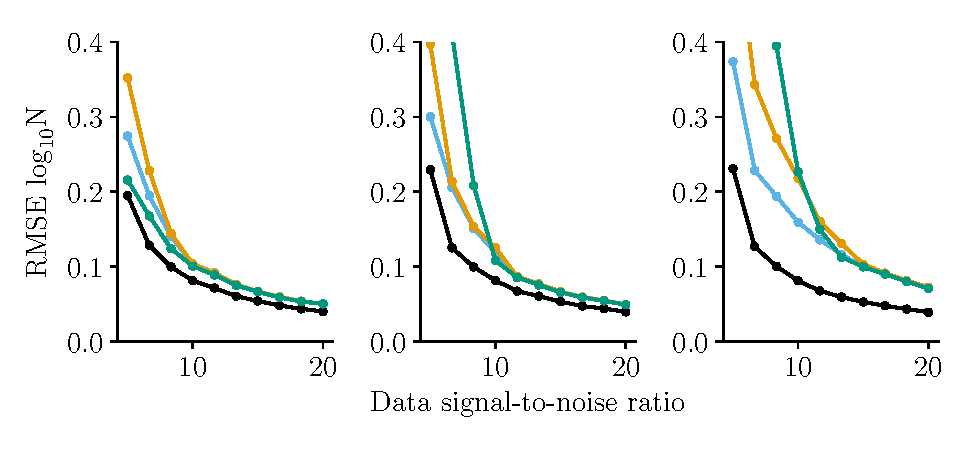
\includegraphics[width=\linewidth]{figures/marginalized_unmarginalized_labeled.pdf}
  \caption{
  Accuracy and precision of different methods of measuring the column density of a single line superimposed on a continuum with known parametrization.
  The accuracy/precision is defined in terms of the root mean square error (RMSE) of the logarithm of column density measurements.
  The signal-to-noise ratios (SNRs) of the artifically generated spectra used for this test are shown on the x-axis of each panel.
  The panels correspond to different continuum parametrizations, from left to right: 0th order polynomial, 1st order polynomial, 2nd order polynomial.
  The line colors indicate different measurement methods, which are listed in the figure legend.
  These methods are explained in detail in Section \ref{sec:marginalization-over-parameters}.}
  \label{fig:order-known-comparison}
\end{figure}

We consider the problem of measuring the column density of a single well-resolved, unsaturated absorption line superimposed on a continuum whose parametrization is known but whose parameters are not known.
To do this, we generate spectra containing a fixed absorption line with different continuum parametrizations and signal-to-noise ratios (SNRs) and measure the column density from each of these spectra.
The continuum parametrizations we use are polynomials of order 0, 1, and 2.
We consider SNRs between 5 and 25.
The summary statistic that we use to indicate quality is the root mean square error (RMSE) of the base ten logarithm of the column density ($\log_{10}{\rm N}$).
To compute each RMSE, we generate 1000 spectra.
We use the logarithm of the column density because physical constants (e.g. oscillator strengths) cancel in that RMSE calculation.

We measure the column density in four ways: (1) supply the correct continuum parameters and only fit for the absorption line parameters; (2) simultaneously fit for continuum and absorption line parameters; (3) analytically marginalize over continuum parameters and fit for absorption line parameters; and (4) use the absorption line parameters recovered using method (1) to define a line-free spectral region, fit continuum parameters just to this region, and with those continuum parameters fit for the absorption line parameters.
The first method is meant to set a lower limit on the RMSE of $\log_{10}{\rm N}$ as a function of SNR.
The second and third methods are two possible ways of automatically modeling the continuum.
The fourth method is meant to approximate the actions of a human manually analyzing a spectrum.
We assume the human can correctly estimate the continuum by eye, correctly estimate the best-fit absorption line profile by eye given this continuum, and finally use this profile to determine which part of the spectrum is not affected by the line.

The RMSEs obtained using these different methods are shown in Figure \ref{fig:order-known-comparison}.
Above an SNR of 10-15, all methods where the correct continuum parameters are not known a priori are equal.
At and below that SNR range, marginalization has a lower RMSE than both simultaneous fitting and the human-like analysis.
The advantage of marginalization over the other methods becomes greater as the continuum parametrization becomes more complex.

\subsection{Marginalization over parametrizations}
\label{sec:marginalization-over-parametrizations}
\begin{figure}
  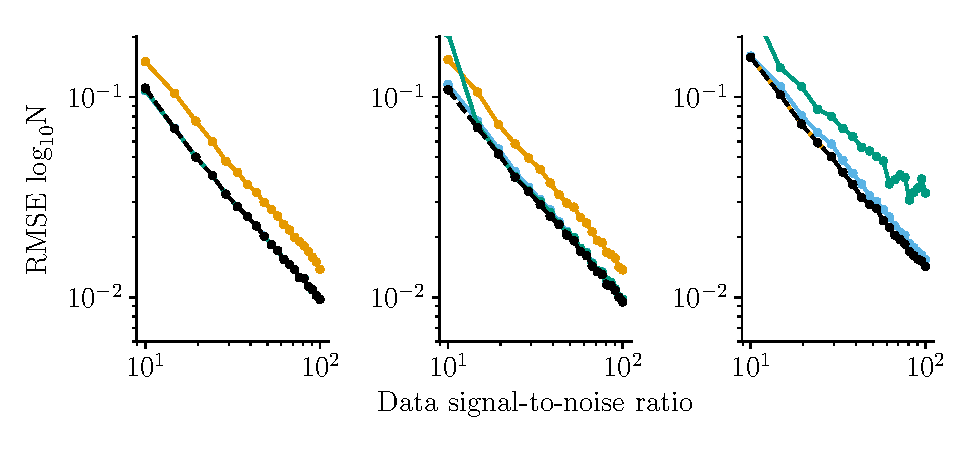
\includegraphics[width=\linewidth]{figures/order_strategies_labeled.pdf}
  \caption{
  Accuracy and precision of different methods of measuring the column density of a single line superimposed on a continuum with unknown parametrization.
  The accuracy/precision is defined in terms of the root mean square error (RMSE) of the logarithm of column density measurements.
  The signal-to-noise ratios (SNRs) of the artifically generated spectra used for this test are shown on the x-axis of each panel.
  The panels correspond to different true continuum parametrizations, from left to right: 0th order polynomial, 1st order polynomial, 2nd order polynomial.
  The line colors indicate different measurement methods, which are listed in the figure legend.
  These methods are explained in detail in Section \ref{sec:marginalization-over-parametrizations}.
  }
  \label{fig:order-unknown-comparison}
\end{figure}
Next, we consider a problem where there is still a single well-resolved and unsaturated absorption line but where we only know that the continuum belongs to a \emph{family} of possible continuum parametrizations.
As in the previous section, we consider three possible continuum parametrizations: 0th, 1st, and 2nd order polynomials.
The approach, simulating spectra, measuring $\log_{10}N$ for each simulated spectrum, and computing the RMSE of $\log_{10}N$, is also the same.
However, we consider a different range in SNR: 10 to 100.

We measure the column density in three ways: (1) supply the correct parametrization and marginalize over its parameters; (2) assume the most complicated of the three parametrizations and marginalize over the parameters; (3) repeatedly use the likelihood ratio test to choose a parametrization and fit for parameters; (4) marginalize over parametrizations as well as parameters.
Method (1) is meant to establish a reference minimum RMSE for this test case.
Method (2) is a conservative assumption that can be made when the family of possible parametrizations is nested---a polynomial of order $n$ with leading coefficient 0 is a polynomial of order $n-1$.
Methods (3) and (4) are different ways of automatically accounting for the different possible parametrizations, in one case (3) by selecting a parametrization and in other (4) by averaging over parametrizations.
The likelihood function that we maximize when using method (4) is the weighted sum of the continuum-marginalized likelihoods of the three possible models.
The weights are the prior probabilities of each of the models; we assume all three are equally likely.

The RMSEs of the four methods are shown in Figure \ref{fig:order-unknown-comparison}.
Three ways of interpreting results. Robustness of solution to decrease in SNR and shortening of spectrum relative to number of parameters; RMSE obtainable by different methods at fixed SNR; SNR required by different methods to obtain the same SNR.
 By robustness, we mean that RMSE has a consistent scaling with SNR and true continuum order.
The estimator does not break down as SNR decreases below some breakdown point or as the number of continuum parameters increases.
The reference, conservative, and parametrization-marginalization methods are robust for SNRs between 10 and 100.
On the other hand, the parametrization-selection method is not robust; its RMSE blows up at an SNR of 10 for spectra with 1st order continua and at all SNRs considered for 2nd order continua.
Parametrization selection should not be used for noisy spectra or spectra with a high ratio of parameters to data points.

In terms of RMSE, the parametrization-marginalized estimator is nearly as good as the reference estimator.
The ratio RMSE$\textrm{m}$/RMSE$\textrm{r}$ of the parametrization-marginalized RMSE, RMSE$\textrm{m}$, to the reference RMSE, RMSE$\textrm{r}$, is 1, 1.04, and 1.1 for spectra with 0th, 1st, and 2nd order continua.
For spectra with 0th or 1st order continua, the conservative estimator is significantly worse than the reference estimator.
RMSE$\textrm{c}$/RMSE$\textrm{r}$ is 1.5, 1.5, and 1, respectively, where RMSE$\textrm{c}$ is the RMSE of the conservative estimator.
These ratios are approximately constant across the entire SNR range considered.
When analyzing an already acquired sample of observations in which a variety of continuum parametrizations are present, using the parametrization-marginalization estimator rather than the conservative estimator will, on average, yield higher accuracy and precision.

To get a sense of how much better the parametrization-marginalization estimator is than the conservative estimator, we can look at the SNR the two estimators require to achieve the same RMSE.
For spectra with 0th, 1st, and 2nd continua, the ratio of the required SNRs SNR$\textrm{c}$/SNR$\textrm{m}$ is 1.6, 1.5, and 0.9.
These ratios are consistent across the entire considered SNR range.
Assuming that SNR is proportional to the square root of integration time, as is the case for Poisson noise-limited observations, these SNR ratios can be converted to required observing time ratios.
Reaching the RMSE of the parametrization-marginalized estimator with the conservative estimator takes 1.26, 1.22, and 0.95 times as much observing time.
When designing an observing strategy to meet a column density RMSE requirement, using the parametrization-marginalized estimator rather than the conservative estimator can save observing time given a fixed sample or increase the size of a sample given a fixed amount of observing time.

\subsection{MCMC efficiency}
\label{sec:multiple-absorption-line-test-case}

\begin{figure}
  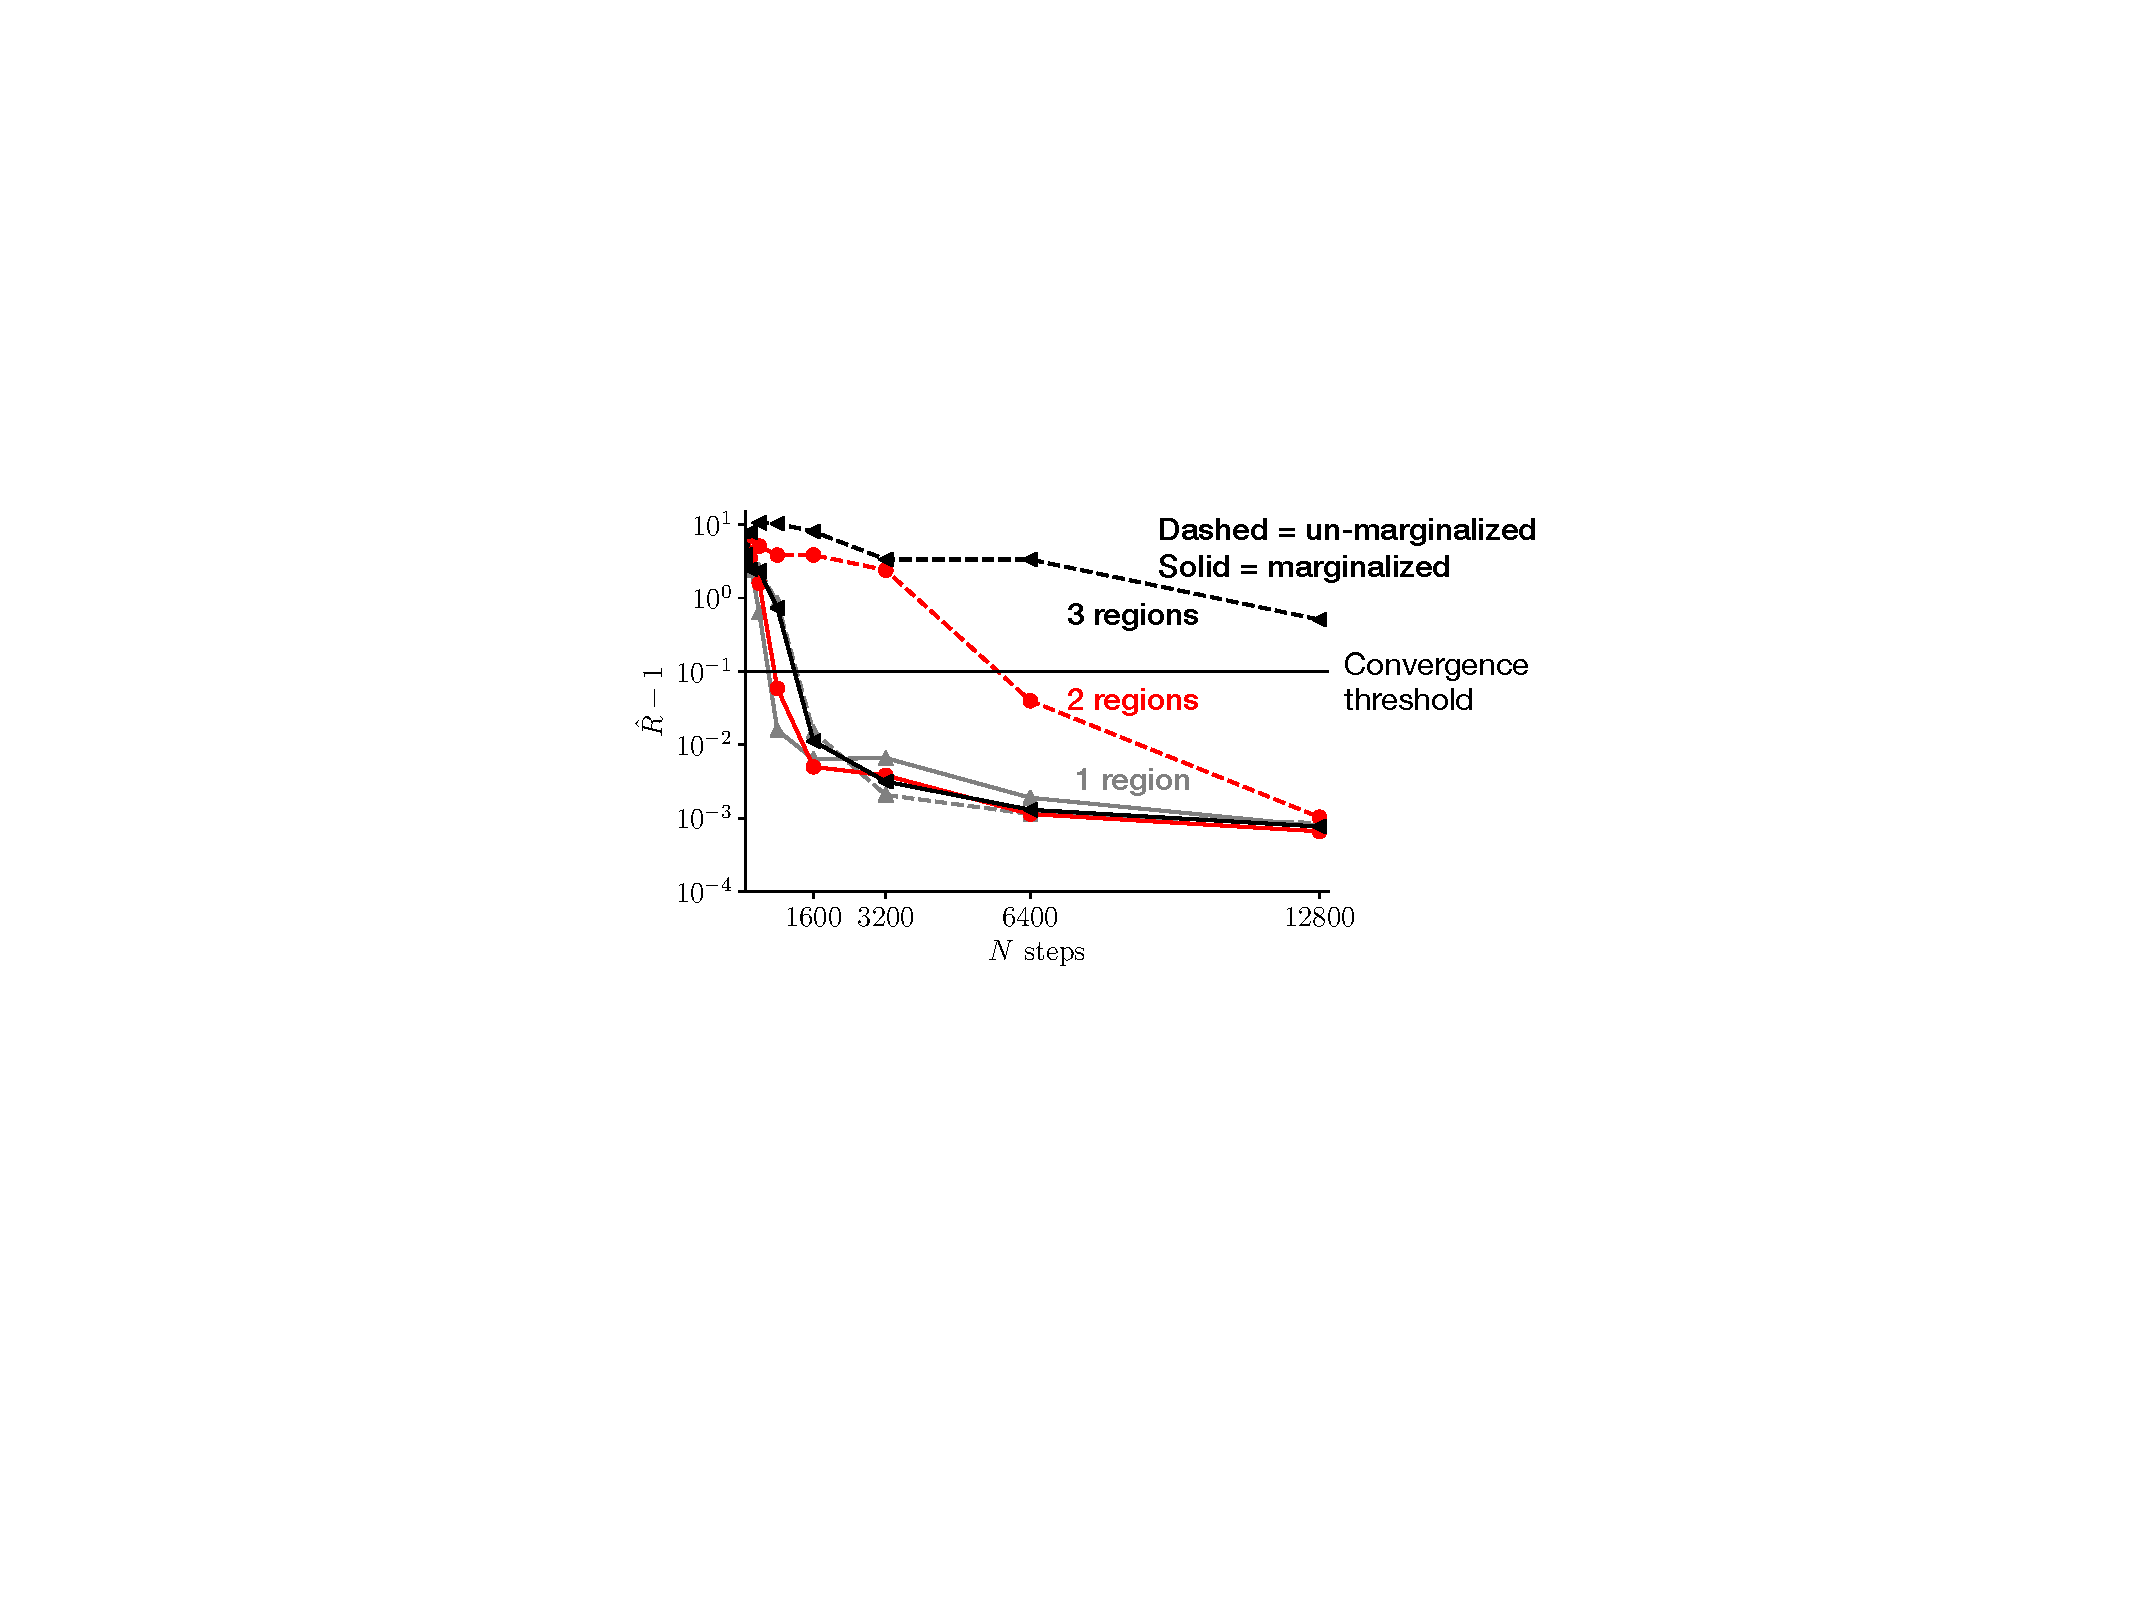
\includegraphics{convergence.pdf}
  \caption{
  Convergence rate of MCMC with analytic and numerical continuum parameter marginalization for absorption line analysis problems with different complexities.
  The convergence diagnostic (y-axis) is the Rubin-Gelman statistic, an estimate of how much smaller the Monte Carlo error of an MCMC-based parameter estimate can get.
  Each line shows the evolution of this convergence diagnostic as a function of the number of MCMC steps taken (x-axis).
  Line styles indicates whether continuum parameters are marginalized over analytically (solid) or included in MCMC (dashed).
  Line colors and markers indicate the number of spectral regions, each of which has its own set of continuum parameters, are being analyzed simultaneously.
  The Rubin-Gelman statistic and the problem setup are discussed in more detail in Section \ref{sec:multiple-absorption-line-test-case}.
  }
  \label{fig:convergence-comparison}
\end{figure}

\begin{figure}
  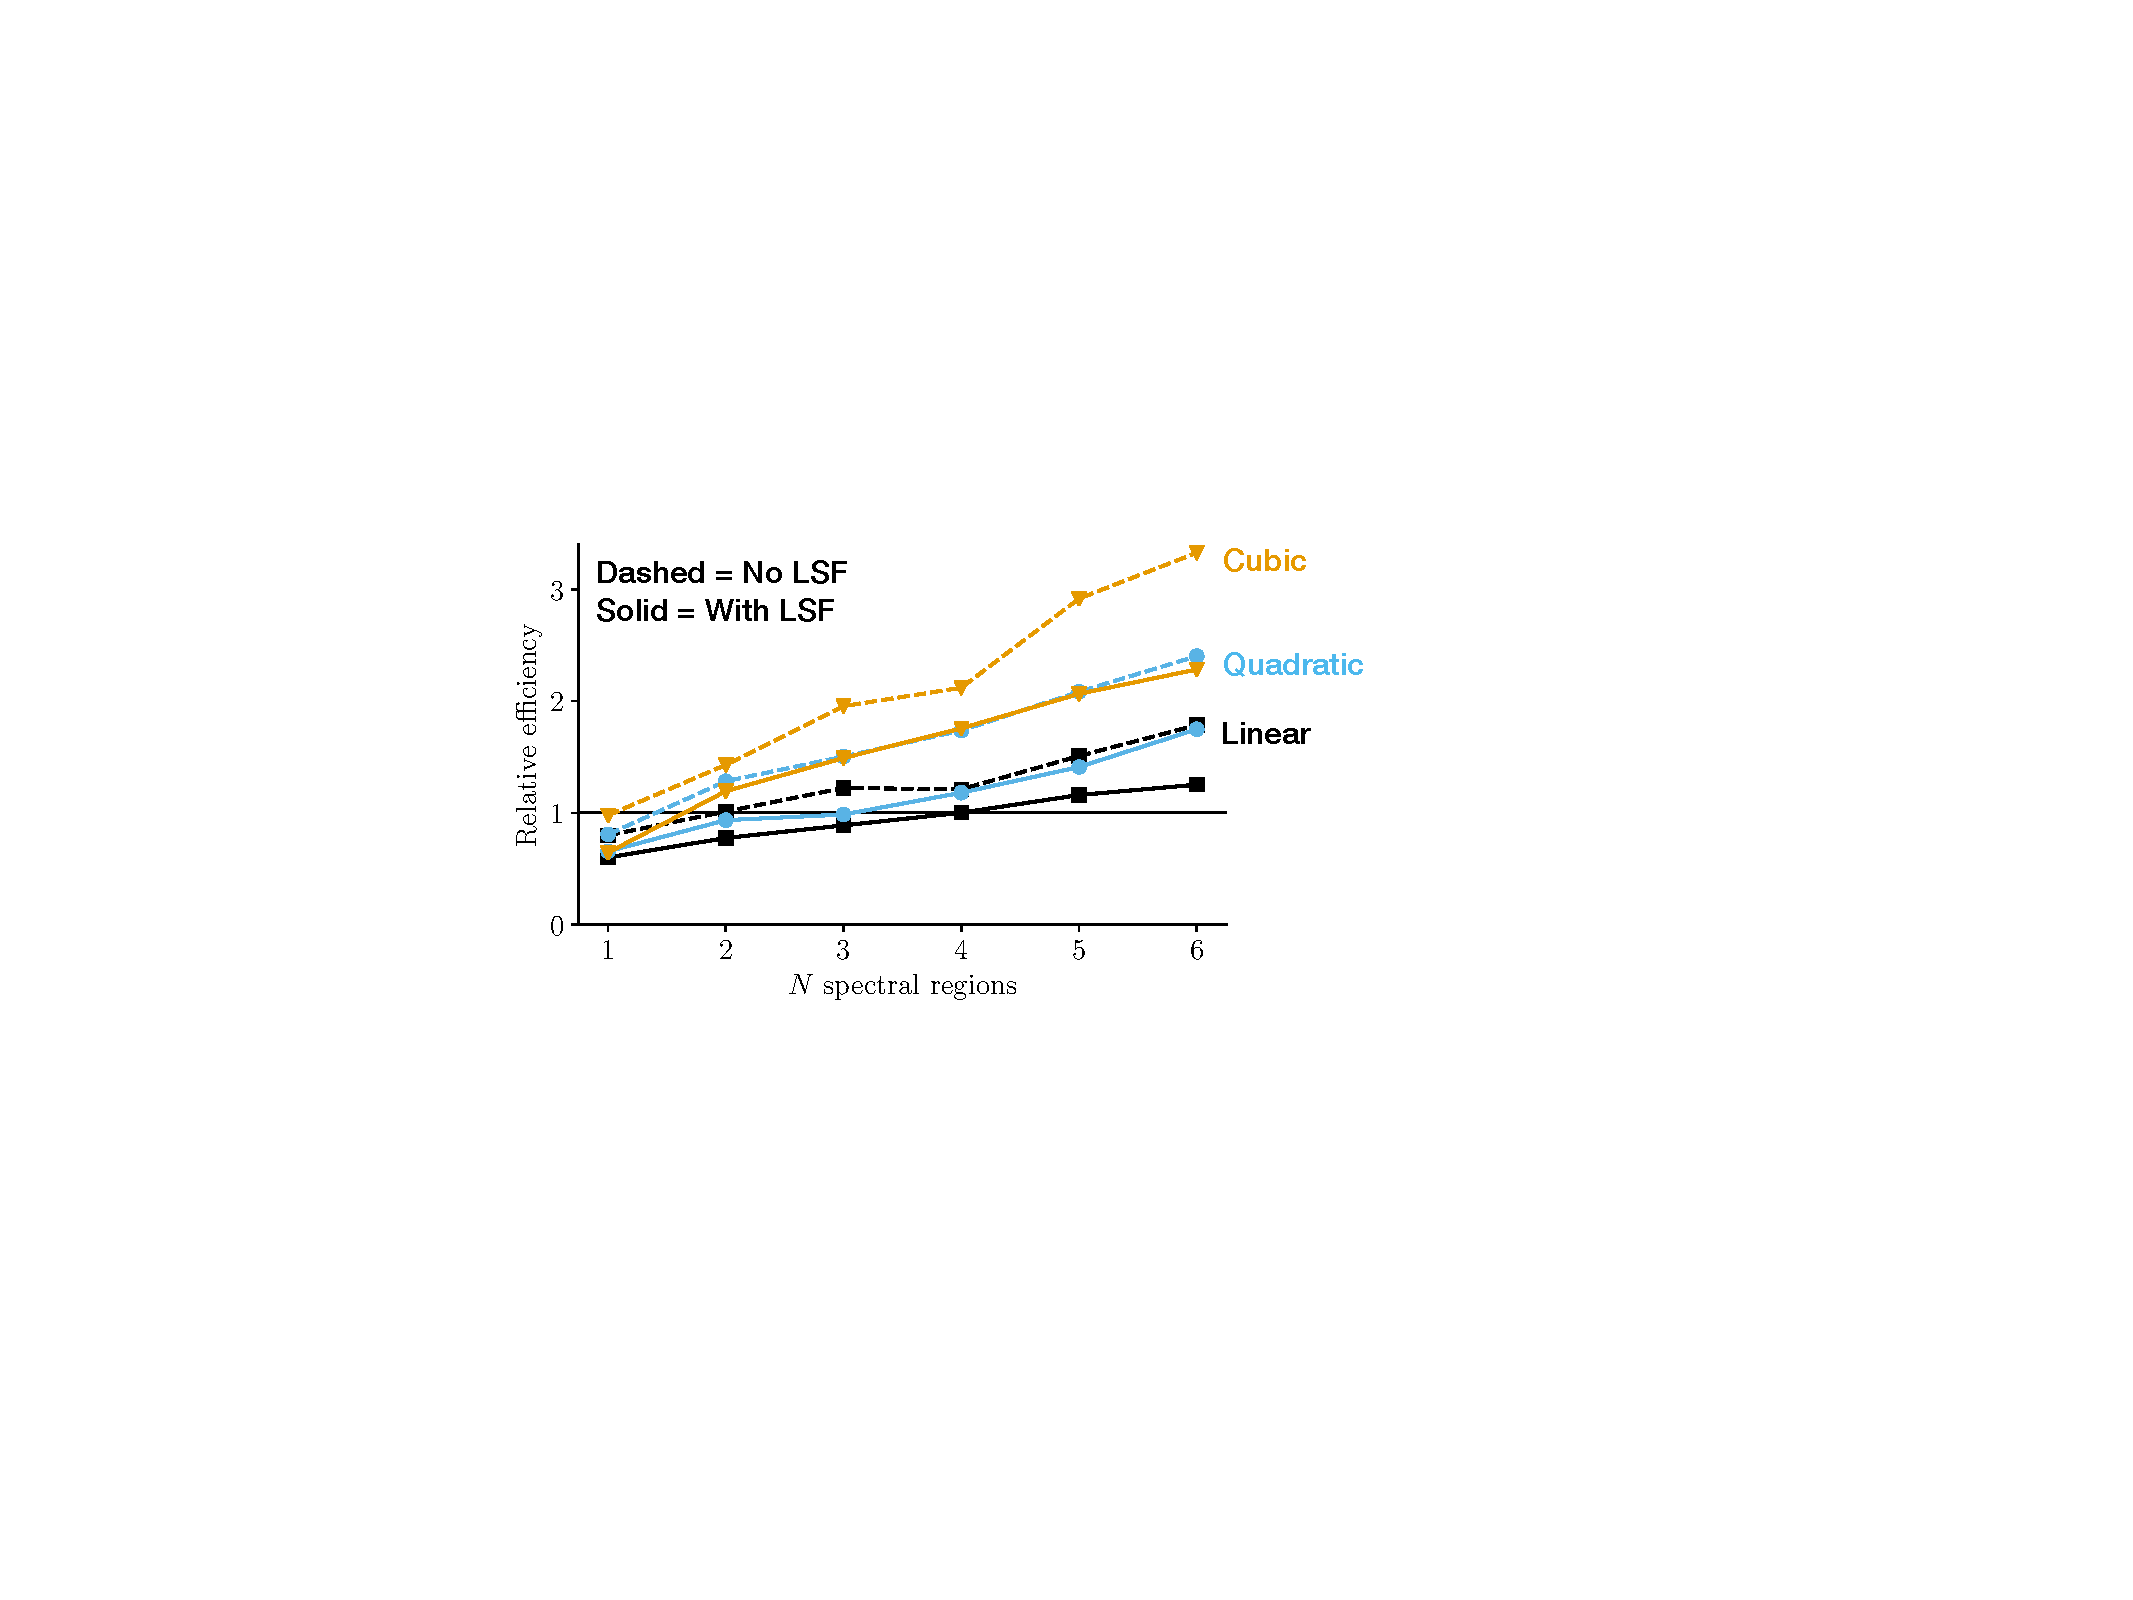
\includegraphics{efficiency.pdf}
  \caption{
  Relative efficiency of MCMC with analytic and numerical continuum parameter marginalization for absorption line analysis problems with different complexities.
  The relative efficiency is the ratio of the number of independent samples generated in the same amount of time by the two marginalization approaches.
  The larger the relative efficiency, the more independent samples generated by analytic marginalization.
  Line colors and markers correspond to different continuum parametrizations: 1st order polynomial (black squares), 2nd order polynomial (blue circles), 3rd order polynomial (orange triangles).
  Line styles indicate whether a non-trivial line spread function (LSF) is used in the analysis.
  The relative efficiency is shown as a function of the number of spectral regions being analyzed simultaneously; each spectral region has its own set of continuum parameters.
  The relative efficiency and the problem setup are discussed in more detail in Section \ref{sec:multiple-absorption-line-test-case}.
  }
  \label{fig:efficiency-comparison}
\end{figure}

In ISM absorption spectra, it is common to have multiple lines in a spectrum with shared parameters
These lines can be from the same species, e.g. the Lyman series, or from different species, e.g. from Mg\small{I}, Zn\small{II}, and Cr\small{II} in the near ultraviolet.
When these lines are in different regions in a spectrum, each region needs its own continuum parameters; this is the case in which BayesVP does not allow the inclusion of continuum parameters in inference.
This is one of the scenarios in which analytic marginalization can be more efficient than MCMC marginalization.

We compare the two methods on how quickly MCMC done using each converges and how efficient MCMC done using each is post-convergence.
Which comparison is more informative for choosing which method to use will depend on the purpose of the MCMC run.
If the goal of an MCMC run is to estimate some value at low-to-moderate precision, the rate of convergence will be the more important factor.
If the goal is to estimate some value at high precision, the burn-in period will usually be a small fraction of the total chain and post-convergency efficiency will be more important.

We consider a case where there are $N$ absorption lines with shared velocity structure, i.e. central velocity and velocity width, but with different amplitudes.
Each absorption line is in a different spectral region.
The continuum in each spectral region is a polynomial of order $M$.
The marginalized likelihood has $2 + N$ absorption line parameters.
The unmarginalized likelihood has $2 + N$ absorption line parameters and $N \times M$ continuum parameters.
We use the \texttt{emcee} implementation of the Goodman and Weare affine-invariant MCMC ensemble sampler to generate draws from the posterior corresponding to each of these likelihoods.
We use the minimum number of `walkers,` which is twice the number of parameters.

We use the Rubin-Gelman statistic $\hat{R}$ CITEP to assess convergence.
- TKTK WHAT IS THE RUBIN-GELMAN STATISTIC
We run ten MCMC instances for 12800 (per-walker) steps and compute the Rubin-Gelman statistic from the second half of sub-chains of length $2^p \times 100$ for $p=0, 1, \ldots, 7$.
$\hat{R}$ is computed separately for each parameter.
Following common usage, we consider convergence to be reached when the $\hat{R}$ of all parameters is less than $1.01$.
We run this test for 1, 2, and 3 regions and absorption lines assuming a continuum of order 1, i.e. a straight line.
The value of the $\hat{R}$ as a function of (total) number of steps is shown in Figure \ref{fig:convergence-comparison}.
When there is a single region and line, the MCMC marginalization chain takes twice as many steps as the analytic marginalization chain to converge; when there are two regions, it takes eight times as many steps; when there are three, the MCMC marginalization chain has not converged by the maximum chain length of 12800 while the analytic marginalization chain converges within 1600 steps.

We use the number of independent samples per unit time to assess efficiency.
We run MCMC with the marginalized likelihood for 2000 burn-in steps and 8000 converged steps and record the average time per sample, $t_s$
Because MCMC with the unmarginalized likelihood takes many steps to converge, we use draws from the converged part of the marginalized likelihood chain as a starting point
These draws only have values for the absorption line parameters
At each set of absorption line parameters, we sample a set of continuum parameters from the conditional distribution discussed in Section \ref{subsec:conditionals}
From this starting point, we run MCMC with the unmarginalized likelihood for 4000 burn-in steps and 36000 converged steps and record the average (wall) time per sample
We then compute the average integrated autocorrelation times $\tau_f$ of the walkers in both chains.
The number of independent samples per unit time is $n_i = \left(\tau_f \, t_s \right)^{-1}$.

We compute $n_i$ for a number of regions $N = 1, 2, \ldots, 6$, continua of polynomial order $M=$ 1, 2, and 3, and either a trivial LSF or a banded LSF.
The ratio $n_i^{\text{marg}} / n_i^{\text{unmarg}}$ for each of these cases is shown in Figure \ref{fig:efficiency-comparison}.
When this ratio is greater than 1, running MCMC with the marginalized likelihood for a fixed amount of time will produce more independent samples than running MCMC with the unmarginalized likelihood for the same amount of time.
The greater the number of regions and the order of the continuum, the greater the efficiency advantage of the marginalized likelihood over the unmarginalized likelihood.
This advantage will not depend on the number of datapoints in each spectral region so long as the LSF is trivial or banded, since the evaluation time of both likelihoods grows linearly with dataset length (see Section \ref{subsec:scaling}).


\section{Discussion}
\label{sec:discussion}
\subsection{Assumptions and consequences}
The explicit assumptions of our analytic marginalization method are that the continuum is a linear function, that the coefficients of this linear function are unconstrained, that uncertainties in the observations are (possibly multivariate) Gaussian, and that the covariance matrix of this Gaussian does not depend on the continuum.
These assumptions obviously do not strictly hold for any dataset.
For example, unconstrained coefficients never hold because no background source produces negative flux; this is largely irrelevant in practice.
A more relevant example is data in the low photon count regime, which are better described by a Poisson distribution than a Gaussian distribution.
This is particularly important when the uncertainties on the measurements are themselves highly uncertain and should be explicitly modeled.
In that case, the uncertainties will depend on the Poisson intensity function, which explicitly depends on the continuum.
Analytic marginalization of the kind described in this work should not be applied to low SNR X-ray or UV spectra.

The continuum models envisaged in this work will usually be effective descriptions rather than (often non-linear) physical descriptions.
Most continua whose variation is over longer wavelength scales than the width of absorption lines in question can be approximated in this way.
Examples of background sources whose continua can be accurately described in this way include quasars and (particularly rapidly rotating) hot stars.
With flexible linear models such as splines, it is possible to describe somewhat complicated pseudo-continua such as stellar wind lines.
For even more complicated pseudo-continua such as those of cool stars \citep[e.g.]{Zasowski:2015hi}, it is necessary to use a non-linear model.
Marginalizable linear models can still be useful even in this case as a way of introducing small corrections for pseudo-continuum features that are not perfectly described by the non-linear model.

An assumption that is not necessary for analytic marginalization to be possible but is necessary for it to be useful is that the absorption model can correctly describe the actually present absorption.
If a region of a spectrum contains two clearly distinct absorption lines but the model one allows for a single line, the presence of the un-modeled line will bias the continuum model.
In short, improvements in continuum modeling cannot solve problems of model misspecification.

\subsection{Interpreting the test cases/the possibilities opened up by analytic marginalization}
The test cases in Section \ref{sec:test-cases} showed that marginalization over continuum parameters and parametrizations is more precise, accurate, and robust than the alternatives.
These results agree with a number of recent works that tout (HMM) the usefulness of (numerical) parameter marginalization in absorption line fitting \citep{2017ApJ...844..136E} (OTHERS).
On its own, analytic marginalization is just a potentially more computationally efficient way of implementing an existing inference approach.
It also allows two qualitatively new approaches: continuum model averaging and absorption parameter optimization with a continuum-marginalized likelihood function.

The test case in Section \ref{sec:marginalization-over-parametrizations} combines both of these approaches---optimizing an absorption parameter likelihood function where the parametrization and parameters of the continuum have been marginalized over.
Analytic marginalization makes this possible in two ways: availability of closed form likelihoods and availability of gradients of closed form likelihoods.
This is useful for dealing with large surveys.
Analyses of absorption lines in tens of thousands of spectra \citep[e.g.]{2013ApJ...770..130Z,Zasowski:2015hi} cannot practically be done with MCMC.
With analytic marginalization, it is possible to at least marginalize over continuum parameters.
The results of the test cases suggest that this approach could mean a non-trivial improvement in the accuracy and precision of absorption line measurements.

In cases where MCMC is possible, combining continuum parametrization marginalization with a probabilistic specification of absorption component structure would allow absorption line analysis with human intervention only at the level of specifying priors and candidate continuum parametrizations.
Component structure specification can be done in a trans-dimensional inference framework, in which the dimensionality of parameter space (in this case the number of sets of absorption line parameters) is itself a parameter of the model.
This way of doing absorption line analysis has two potential advantages.
Because it includes marginalization over many different nuisance parameters, it should be pretty robust (e.g. to unresolved saturated structure).
Because it is essentially automatic, it allows blinding, which is good for hypothesis testing, and improves reproducibility.

\section{Conclusion}
\label{sec:conclusion}
have a package that computes marginal likelihoods and their gradients
idea of marginalizing over linear parameters is not new, but to best of our knowledge had not been applied to problem of absorption line continua.
there are some problem-specific features, e.g. LSFs, which can be handled more efficiently with a purpose-built package.

have carried out tests on whether continuum marginalization is any better than several simpler approaches.
 have shown that in terms of accuracy of recovered parameters, marginalization is best way of doing "simple," "local" continua.
true on two levels: if you have a good guess as to the correct parametrization, marginalizing over the parameters will, at low SNR, get you more accurate parameter recovery.
if you only have a good guess as to the set of plausible parametrizations, marginalizing over parametrizations and parameters within each parametrization is almost as good as knowing the correct parametrization.
marginalizing over parametrizations will, on average, yield more accurate parameter values than any of the other strategies we tested. (do I need to test picking a parametrization using a likelihood test?)
this extra accuracy is free! it's like having a higher SNR spectrum and analyzing it in the simpler, less-good way.
this extra accuracy does not require much extra compute and (when line placement is known) can be used automatically, making it great for analysis of data from massive spectroscopic surveys.

have also considered an ``opposite'' case, a single spectrum with many different lines that you want to analyze very carefully with MCMC.
analytic continuum marginalization can dramatically speed up convergence of MCMC and shorten chain autocorrelation times (since there are fewer parameters to deal with numerically).
when there are many continuum parameters to deal with (as is the case when you have a bunch of splines, e.g.), shortening of autocorrelation times can mean more independent samples per second---greater efficiency.

list of results:
\begin{itemize}
  \item likelihood and gradient
  \item package implementing the above
  \item demonstration that continuum marginalization is practically useful in terms of achieving greater accuracy and, in some cases, efficiency
\end{itemize}

\acknowledgments People: Josh Peek, Andrew Fox, Yong Zheng, Andrew Casey, Cameron Liang

\software{emcee \citep{2013PASP..125..306F},
numpy \citep{vanderWalt:dp},
matplotlib \citep{2007CSE.....9...90H}
}

\appendix

\section{Implementation and demonstration}
\label{sec:package-and-demos}
In this Appendix, we describe some capabilities and limitations of the package (Section \ref{subsec:package-functionality}) and show how the computation time of different calculations grows with dataset and basis size (Section \ref{subsec:scaling}).

\subsection{Package functionality}
\label{subsec:package-functionality}
This package was designed for a use case where the log marginal likelihood and its gradient are evaluated at many different values of the $\theta$-dependent parameters while the $\theta$-independent parameters are held constant.
The core feature of the package is the \texttt{MarginalizedLikelihood} class.
A \texttt{MarginalizedLikelihood} instance stores $\theta$-independent parts of the model and pre-computes quantities that are re-used during repeated marginalized likelihood evaluations.
In particular, it stores the data covariance matrix $\vx{K}$; the $\vx{c}$ prior covariance matrix $\vx{\Lambda}$ and its explicit inverse, if applicable; and the line spread function-like linear mapping $\vx{L}$ and its transpose.

Both covariance matrices can be diagonal or fully general.
To ensure a common interface, the package includes the \texttt{CovarianceMatrix} class, which defines an interface that ensures necessary calculations can be done, and two subclasses, \texttt{DiagonalCovarianceMatrix} and \texttt{GeneralCovarianceMatrix}.
\texttt{GeneralCovarianceMatrix} uses the Cholesky decomposition of the supplied covariance matrix for determinant calculations and left multiplication of matrices and vectors by the inverse of the supplied covariance matrix.
Computing the Cholesky decomposition of a general covariance matrix of size $M$ by $M$ takes $\mathcal{O}(M^3)$ calculations, making it prohibitively computationally expensive for large $M$.

The linear mapping $\vx{L}$ can be any object that implements the matrix multiplication interface, i.e. has a \texttt{matmul} or \texttt{\_\_matmul\_\_} method.
For example, $\vx{L}$ can be a dense matrix represented by a \texttt{numpy} array, a sparse matrix represented by a \texttt{scipy.sparse} matrix, or a convolution operator represented by a \texttt{scipy.sparse.linalg} \texttt{LinearOperator}.
$\vx{L}$ can also be the identity mapping (indicated by \texttt{None}), in which case it is left out of any likelihood calculations.


\subsection{Computation time as a function of dataset and basis size}
\label{subsec:scaling}
The most time-consuming step in computing all of the quantities derived in Section \ref{sec:assumptions-and-formalism} is forming the matrix $\vx{C}_{n/u}$.
This step requires matrix-matrix products while most other steps only involve matrix-vector products.
These expensive products are $\vx{L}\vx{B}$ and $\vx{K}^{-1} \left(\vx{L} \vx{B}\right)$.
The amount of time required to compute these products depends on the structure $\vx{L}$ and $\vx{K}$.

$\vx{L}$ can be the identity matrix, a dense matrix, a sparse matrix, or a linear mapping such as convolution.
The fastest case is when $\vx{L}$ is the identity matrix, since then $\vx{L}\vx{B}$ does not need to be computed.
The slowest case is when it is a dense matrix, in which case computation time grows as $\mathcal{O}(MN(P+Q))$.
When $\vx{L}$ is a sparse matrix or linear mapping, the scaling depends on its exact structure.
One case that is relevant to the analysis of spectra is a $\vx{L}$ that represents a line spread function.
A line spread function that varies with wavelength can be represented by a banded matrix, which will be sparse if the spectrum spans many resolution elements.
If the bandwidth of $\vx{L}$ is independent of the size of the dataset, the computation time of this product grows as $\mathcal{O}(M(P+Q))$.

We consider covariance matrices $\vx{K}$ that are either diagonal or general.
If $\vx{K}$ is diagonal, $\vx{K}^{-1} \left(\vx{L} \vx{B}\right)$ requires exactly $M(P+Q)$ multiplications.
When $\vx{K}$ is a general covariance matrix, we decompose it into its Cholesky factors and left-multiply $\vx{L} \vx{B}$ by $\vx{K}^{-1}$ by solving the linear problem $\vx{\vx{L} \vx{B}} = \vx{K} \vx{X}$.
The time needed to factor $\vx{K}$ grows as $\mathcal{O}\left(M^3\right)$ but only needs to be done once per set of observations.
The time needed to solve the linear problem grows as $\mathcal{O}\left(M^2 (P+Q)\right)$.

To empirically confirm these growth rates, we timed how long it takes to evaluate the log-likelihood and its gradient for a range of dataset sizes $M$ and basis sizes $P+Q$ and three $\vx{L}$ and $\vx{K}$ structure scenarios.
The scenarios are: $\vx{L}$ is the identity mapping, $\vx{K}$ is diagonal; $\vx{L}$ is a dense matrix, $\vx{K}$ is general; and $\vx{L}$ is a sparse, banded matrix and $\vx{K}$ is diagonal.
The first two scenarios are the fastest and slowest combination.
The third scenario is more typical for a spectrum; the data uncertainty is diagonal, the line spread function has finite extent.
The evaluation time of the log-likelihood as a function of $M$ and $P+Q$ for these three scenarios is shown in Figures \ref{fig:uncorr-no-L-logp}, \ref{fig:corr-yes-L-logp}, and \ref{fig:uncorr-sparse-L-logp}.
We do not show the evaluation time of the gradient because it behaves in the same way as the evaluation time of the log-likelihood in all three scenarios; the most expensive step of the two calculations is the same.

The dependence of computation time on $M$ and $P+Q$ generally agrees with the predictions based on the two most time-consuming steps.
At low $M$ and in particular at low $P+Q$, the computation time is either overhead-dominated or evenly split between the most time-consuming steps and other steps.
When $M \gtrsim 10^5$, computation time increases faster than expected purely from the growth rate of the required number of operations (see e.g. the left panel of Figure \ref{fig:uncorr-no-L-logp}).
This excess increase is computation time is most likely due to changes in memory bandwidth, as the size of matrix rows and columns increases past the size of the highest-level CPU cache on the laptop used to run these tests.

To put these dataset sizes into context, a Sloan Digital Sky Survey (SDSS) BOSS or APOGEE spectrum contains $\sim 10^3$ pixels, a Hubble Space Telescope Cosmic Origins Spectrograph (HST-COS) spectrum contains $\sim 10^4$ pixels, and a spectrum from an echelle spectrograph such as the Ultraviolet and Visual Echelle Spectrograph on the Very Large Telescope or the Magellan Inamori Kyocera Echelle spectrograph contains $\sim 10^5 - 10^6$ pixels.
The uncertainties associated with these spectra are usually assumed to be diagonal and the line spread functions are acceptably described by sparse, banded matrices, so the computation times given in Figure \ref{fig:uncorr-no-L-logp} and \ref{fig:uncorr-sparse-L-logp} should apply.

\begin{figure}
  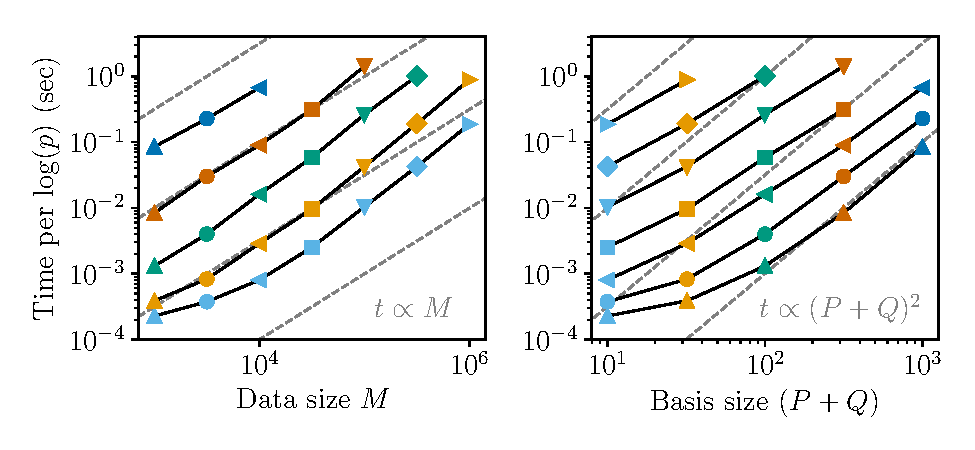
\includegraphics{uncorr_no_L_scaling.pdf}
  \caption{Computation time of the marginal log-likelihood (Equations \ref{eqn:proper-prior-marginal} and \ref{eqn:improper-prior-marginal}) when the data covariance matrix $\vx{K}$ is diagonal and $\vx{L}$ is the identity mapping as a function of dataset size $M$ (left panel) and basis size $P+Q$ (right panel). Values with the same marker shape were computed at the same dataset size $M$. Values with the same marker color were computed at the same dataset size $P+Q$. Polynomials of the form given in the bottom right corner of each panel are shown as dashed gray lines.}
  \label{fig:uncorr-no-L-logp}
\end{figure}

\begin{figure}
  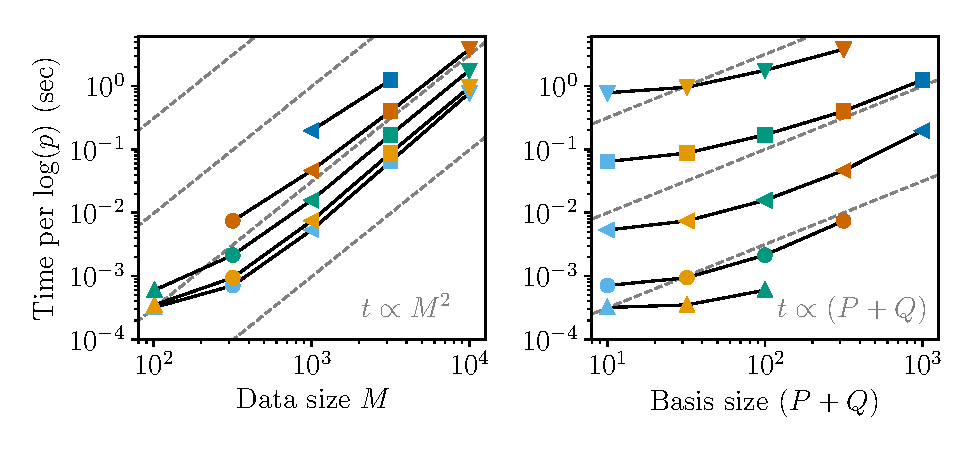
\includegraphics{corr_yes_L_scaling.pdf}
  \caption{Computation time of the marginal log-likelihood when the data covariance matrix $\vx{K}$ is not diagonal and $\vx{L}$ is a dense matrix. See caption of Figure \ref{fig:uncorr-no-L-logp} for a description of figure elements.}
  \label{fig:corr-yes-L-logp}
\end{figure}

\begin{figure}
  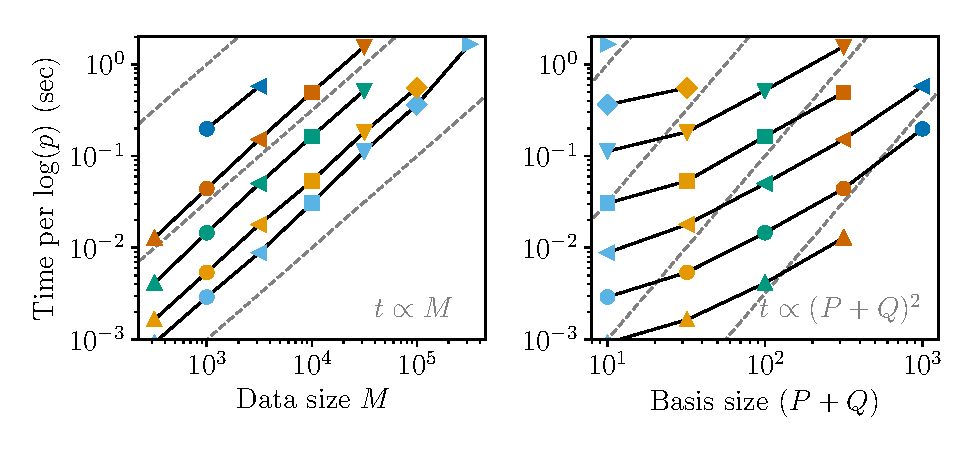
\includegraphics{uncorr_sparse_L_scaling.pdf}
  \caption{Computation time of the marginal log-likelihood when the data covariance matrix $\vx{K}$ is diagonal and $\vx{L}$ is a sparse, banded matrix. See caption of Figure \ref{fig:uncorr-no-L-logp} for a description of figure elements.}
  \label{fig:uncorr-sparse-L-logp}
\end{figure}

\bibliography{bibliography.bib}

\end{document}
